% Chapter Template

\chapter{Theoretical Background and Related Work} % Main chapter title

\label{Chapter2} % Change X to a consecutive number; for referencing this chapter elsewhere, use \ref{ChapterX}
In this section we explain the different types of range measuring in range-based localization systems. For comparison reasons, we shortly introduce variants of received signal strength indication (RSSI), which is the mostly used indoor localization technique. We then briefly explain two slightly less common methods, which were used in our system - two way ranging (TWR) and time difference of arrival (TDOA). We also include some background theory about our implementation and the particle filter.\\
These are the main parts of this section:\\
First a short overview of range based localization with the mean principles of RSSI, TWR and TDOF as well as the concept of triangulation/trilateration and the weighting process. Second we present background information about ultra wideband (UWB) and finally information about the particle filter is given.

%----------------------------------------------------------------------------------------
%	SECTION 1
%----------------------------------------------------------------------------------------

\section{Range based localization}

Range based localization systems are depending on an infrastructure in the area of the localization:
\begin{itemize} 
\item \textbf{Target Node (TAG)} which is the device that is localized. 
\item \textbf{Anchor Nodes (AN)}that are placed on carefully chosen points in the building, to encounter the best coverage of the whole area.
\end{itemize}

\begin{figure}[th]
\centering
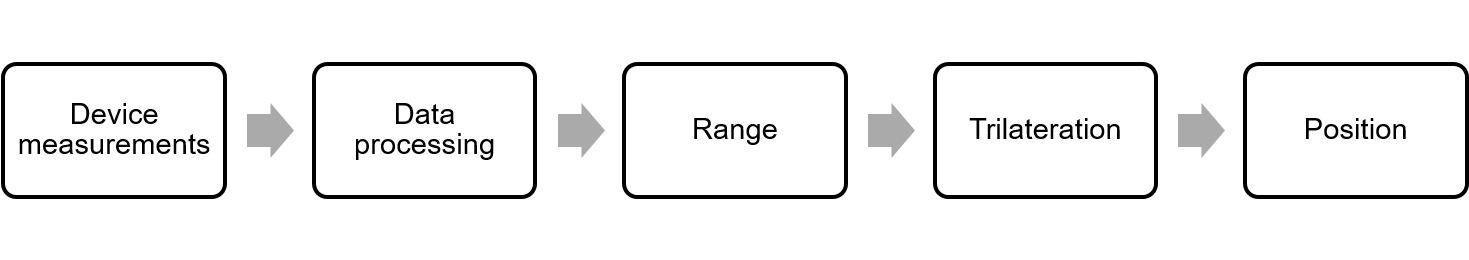
\includegraphics[width=1.0\textwidth]{Figures/ranging_process}
\decoRule
\caption[Ranging process]{A simple ranging process.}
\label{fig:ranging_process}
\end{figure}

As shown in figure \ref{fig:ranging_process}, a simplified localization system work as follows:
Either the TAG, the anchor or both of them collect data used for localization. The data can be a signal strength, a round trip time or IMU measurement.
In a processing unit - on the TAG or on a seperate server - the data is processed and converted into a distance. This is repeated for every anchor node.
The last step contains trilateration of the position using the ranges of every AN to the TAG.

In this abridged scenario, some difficulties are left out. Full indoor localization systems are more complex, as they use ingenious algorithms to improve the accuracy of the estimated ranges or improve the system by adding weighting to deal with incorrect range measures.

%-----------------------------------
%	SUBSECTION 1
%-----------------------------------
\subsection{RSSI and Fingerprinting}




%-----------------------------------
%	SUBSECTION 1
%-----------------------------------
\subsection{Two way ranging, time difference of arrival}



%-----------------------------------
%	SUBSECTION 2
%-----------------------------------
\subsection{Triangulation and Trilateration}
Triagulation and trilateration use the mathematical concepts of triangles to find unknown lengths. Triangulation was already mentioned by the greek mathematician Thales, who used this concept for finding out the height of ancient egypt pyramids. \cite{thales} It was also used for cartography purposes, where angles between fixed points were measured and heights and distances could be calculated. 
Although trilateration and triangulation use the same mathematical triangle concept, they have one defined difference: We call it triangulation, when angles to anchor positions are measured, otherwise - when distances to anchors are measured - it's called trilateration.
As it was easier to measure angles than distances in the past, triangulation was more often used. With modern electronic devices, it is more common to determine distances, rather than angles. 

Figure \ref{fig:trilateration} shows how trilateration is used for positioning. However, this is a theoretical and idealized scenario, where every range can be determined accurately. In real applications, the ranges are not exactly calculated, what leads to the fact that we will not only get a single point for the calculated position, but several points, especially when we use more than three ANs.

\begin{figure}[th]
\centering
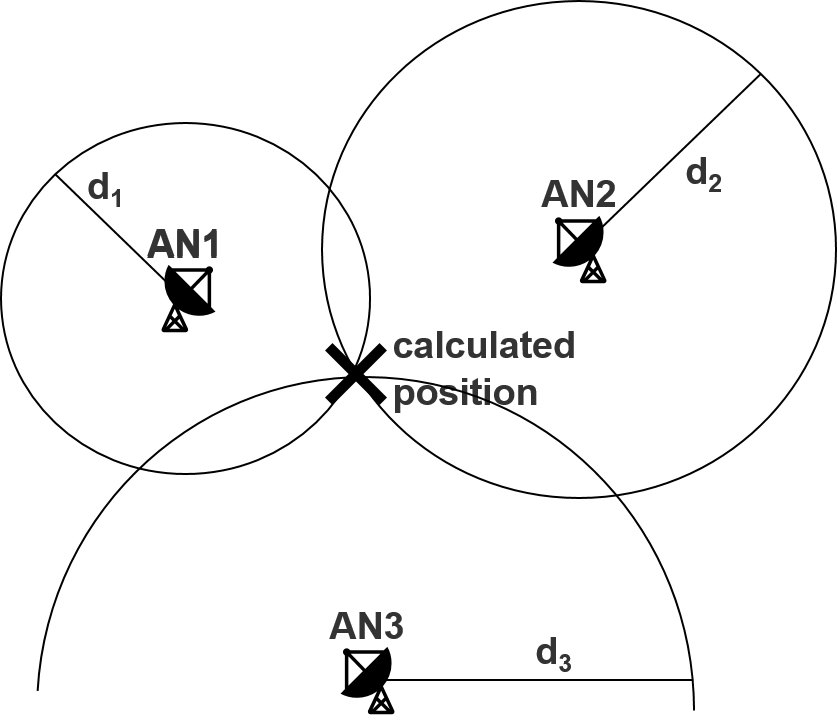
\includegraphics[width=0.6\textwidth]{Figures/trilateration}
\decoRule
\caption[Trilateration]{Graphical illustration of the trilateration concept.}
\label{fig:trilateration}
\end{figure}

%-----------------------------------
%	SUBSECTION 3
%-----------------------------------

\subsection{Weighting}
Morbi rutrum odio eget arcu adipiscing sodales. Aenean et purus a est pulvinar pellentesque. Cras in elit neque, quis varius elit. Phasellus fringilla, nibh eu tempus venenatis, dolor elit posuere quam, quis adipiscing urna leo nec orci. Sed nec nulla auctor odio aliquet consequat. Ut nec nulla in ante ullamcorper aliquam at sed dolor. Phasellus fermentum magna in augue gravida cursus. Cras sed pretium lorem. Pellentesque eget ornare odio. Proin accumsan, massa viverra cursus pharetra, ipsum nisi lobortis velit, a malesuada dolor lorem eu neque.

%----------------------------------------------------------------------------------------
%	SECTION 2
%----------------------------------------------------------------------------------------

\section{UWB Theory}

Sed ullamcorper quam eu nisl interdum at interdum enim egestas. Aliquam placerat justo sed lectus lobortis ut porta nisl porttitor. Vestibulum mi dolor, lacinia molestie gravida at, tempus vitae ligula. Donec eget quam sapien, in viverra eros. Donec pellentesque justo a massa fringilla non vestibulum metus vestibulum. Vestibulum in orci quis felis tempor lacinia. Vivamus ornare ultrices facilisis. Ut hendrerit volutpat vulputate. Morbi condimentum venenatis augue, id porta ipsum vulputate in. Curabitur luctus tempus justo. Vestibulum risus lectus, adipiscing nec condimentum quis, condimentum nec nisl. Aliquam dictum sagittis velit sed iaculis. Morbi tristique augue sit amet nulla pulvinar id facilisis ligula mollis. Nam elit libero, tincidunt ut aliquam at, molestie in quam. Aenean rhoncus vehicula hendrerit.

%----------------------------------------------------------------------------------------
%	SECTION 2
%----------------------------------------------------------------------------------------

\section{Particle Filter}

Sed ullamcorper quam eu nisl interdum at interdum enim egestas. Aliquam placerat justo sed lectus lobortis ut porta nisl porttitor. Vestibulum mi dolor, lacinia molestie gravida at, tempus vitae ligula. Donec eget quam sapien, in viverra eros. Donec pellentesque justo a massa fringilla non vestibulum metus vestibulum. Vestibulum in orci quis felis tempor lacinia. Vivamus ornare ultrices facilisis. Ut hendrerit volutpat vulputate. Morbi condimentum venenatis augue, id porta ipsum vulputate in. Curabitur luctus tempus justo. Vestibulum risus lectus, adipiscing nec condimentum quis, condimentum nec nisl. Aliquam dictum sagittis velit sed iaculis. Morbi tristique augue sit amet nulla pulvinar id facilisis ligula mollis. Nam elit libero, tincidunt ut aliquam at, molestie in quam. Aenean rhoncus vehicula hendrerit.